\begin{center}
  \Large
  \textbf{BIOGRAFI PENULIS}
\end{center}

\addcontentsline{toc}{chapter}{BIOGRAFI PENULIS}

\vspace{2ex}

\begin{wrapfigure}{L}{0.3\textwidth}
  \centering
  \vspace{-3ex}
  % Ubah file gambar berikut dengan file foto dari mahasiswa
  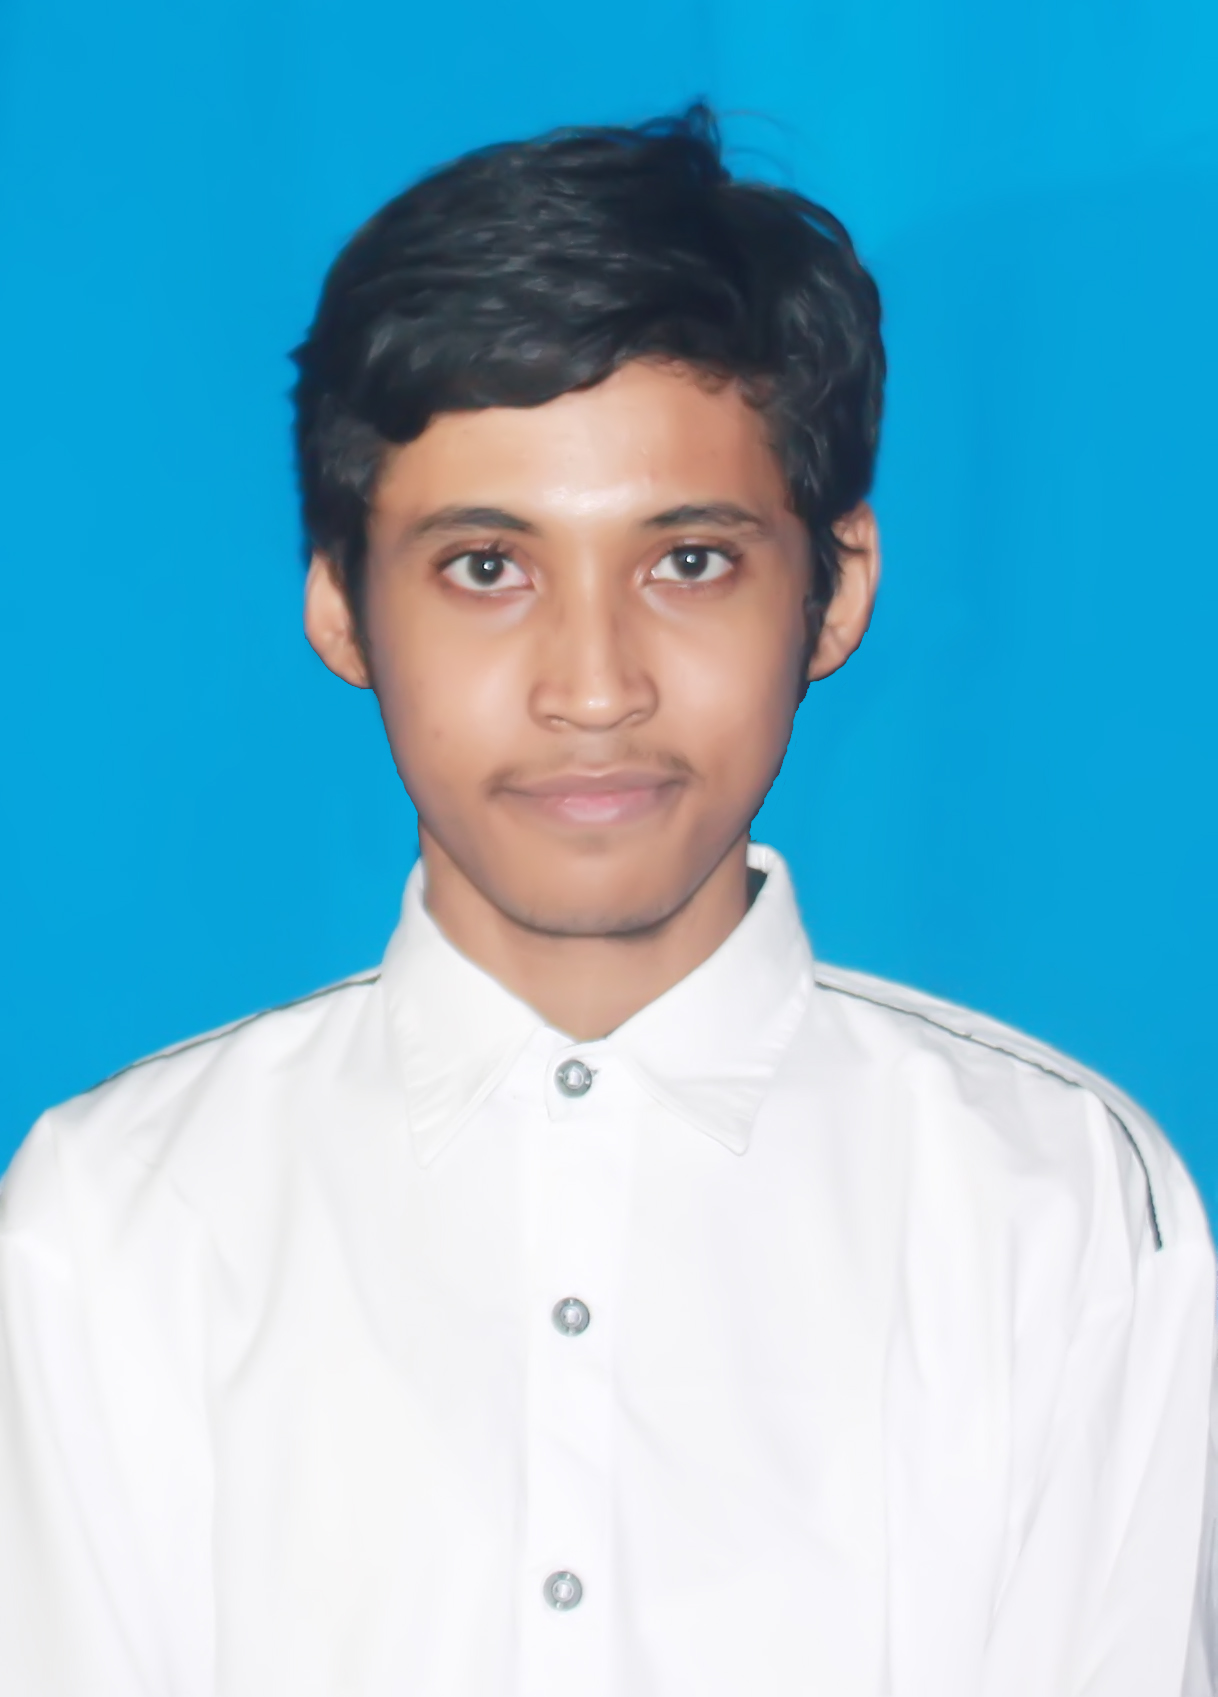
\includegraphics[width=0.3\textwidth]{gambar/portrait.JPG}
  \vspace{-4ex}
\end{wrapfigure}

% Ubah kalimat berikut dengan biografi dari mahasiswa
Dafa Fidini Asqav, biasa dipanggi Fidini dalam kampus ITS, lahir di kota Solo, Jawa Tengah
pada 8 Desember 1999. Penulis mengenyam pendidikan pra kuliah dan hidup sepenuhnya di Solo
sebelum berpindah ke Surabaya untuk melanjutkan studi di jurusan Teknik Komputer Institut Teknologi
Sepuluh Nopember. Sejak sebelum memasuki kuliah, penulis sudah tertarik akan teknologi AI.
Semenjak masa kuliah, penulis terlibat penuh dalam dua \emph{open source project} berupa simulator
untuk \emph{World of Warcraft Classic}, game yang penulis sering mainkan. \emph{Project} tersebut adalah
\url{https://github.com/wowsims/} dan \url{https://github.com/TheGroxEmpire/TBC_DPS_Warrior_Sim}.
Penulis juga saat ini terlibat dalam sebuah modding project \emph{Guardian of Azeroth 2} untuk
game \emph{Crusader Kings 3} sebagai \emph{Senior Tester} \url{https://github.com/Warcraft-GoA-Development-Team/Warcraft-Guardians-of-Azeroth-2/}.